\section{Thống kê mô tả}
\subsection*{4.1 Phân tích và phân chia số liệu}
Sau khi thực hiện bước tiền xử lí số liệu, ta đã làm sạch và điền khuyết dữ liệu, ta thực hiện thống kê mô tả bằng lệnh \texttt{summary()} ta sẽ có cái nhìn tổng quát hơn về bảng dữ liệu. Lệnh \texttt{summary()} sẽ xuất ra màn hình những giá trị như \textit{min} (giá trị nhỏ nhất), \textit{mean} (trung bình), \textit{median} (trung vị), \textit{Q1} (khoảng tứ phân vị thứ 1), \textit{Q3} (khoảng tứ phân vị thứ 3), \textit{max} (giá trị lớn nhất).
\begin{figure}[H]
    \centering
    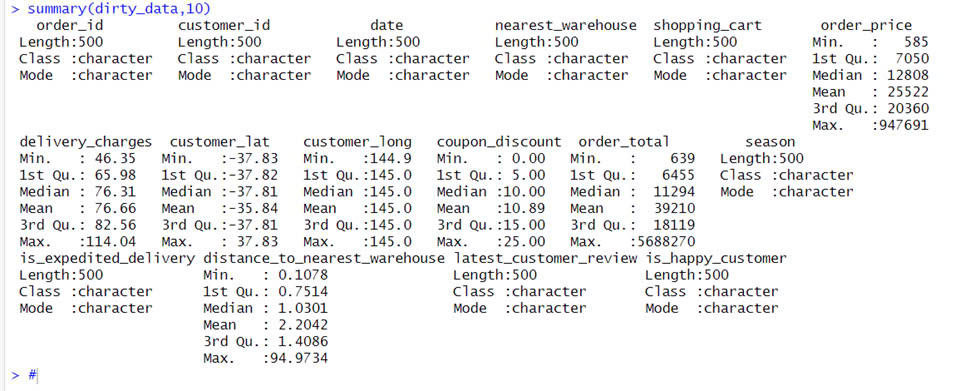
\includegraphics[width=0.9\linewidth]{graphics/bang1.jpg}
\end{figure}